% This is "sig-alternate.tex" V2.0 May 2012
% This file should be compiled with V2.5 of "sig-alternate.cls" May 2012
%
% This example file demonstrates the use of the 'sig-alternate.cls'
% V2.5 LaTeX2e document class file. It is for those submitting
% articles to ACM Conference Proceedings WHO DO NOT WISH TO
% STRICTLY ADHERE TO THE SIGS (PUBS-BOARD-ENDORSED) STYLE.
% The 'sig-alternate.cls' file will produce a similar-looking,
% albeit, 'tighter' paper resulting in, invariably, fewer pages.
%
% ----------------------------------------------------------------------------------------------------------------
% This .tex file (and associated .cls V2.5) produces:
%       1) The Permission Statement
%       2) The Conference (location) Info information
%       3) The Copyright Line with ACM data
%       4) NO page numbers
%
% as against the acm_proc_article-sp.cls file which
% DOES NOT produce 1) thru' 3) above.
%
% Using 'sig-alternate.cls' you have control, however, from within
% the source .tex file, over both the CopyrightYear
% (defaulted to 200X) and the ACM Copyright Data
% (defaulted to X-XXXXX-XX-X/XX/XX).
% e.g.
% \CopyrightYear{2007} will cause 2007 to appear in the copyright line.
% \crdata{0-12345-67-8/90/12} will cause 0-12345-67-8/90/12 to appear in the copyright line.
%
% ---------------------------------------------------------------------------------------------------------------
% This .tex source is an example which *does* use
% the .bib file (from which the .bbl file % is produced).
% REMEMBER HOWEVER: After having produced the .bbl file,
% and prior to final submission, you *NEED* to 'insert'
% your .bbl file into your source .tex file so as to provide
% ONE 'self-contained' source file.
%
% ================= IF YOU HAVE QUESTIONS =======================
% Questions regarding the SIGS styles, SIGS policies and
% procedures, Conferences etc. should be sent to
% Adrienne Griscti (griscti@acm.org)
%
% Technical questions _only_ to
% Gerald Murray (murray@hq.acm.org)
% ===============================================================
%
% For tracking purposes - this is V2.0 - May 2012
\documentclass{sig-alternate}
\usepackage{blindtext}
%\usepackage[showframe]{geometry}
\usepackage{graphicx}
\usepackage{url}
\usepackage{listings}
\usepackage{fancyvrb}
\usepackage{float}

\begin{document}
\title{BaseFS -\\ Basically Available, Soft State, Eventually Consistent Filesystem for Cluster Management}
%
% You need the command \numberofauthors to handle the 'placement
% and alignment' of the authors beneath the title.
%
% For aesthetic reasons, we recommend 'three authors at a time'
% i.e. three 'name/affiliation blocks' be placed beneath the title.
%
% NOTE: You are NOT restricted in how many 'rows' of
% "name/affiliations" may appear. We just ask that you restrict
% the number of 'columns' to three.
%
% Because of the available 'opening page real-estate'
% we ask you to refrain from putting more than six authors
% (two rows with three columns) beneath the article title.
% More than six makes the first-page appear very cluttered indeed.
%
% Use the \alignauthor commands to handle the names
% and affiliations for an 'aesthetic maximum' of six authors.
% Add names, affiliations, addresses for
% the seventh etc. author(s) as the argument for the
% \additionalauthors command.
% These 'additional authors' will be output/set for you
% without further effort on your part as the last section in
% the body of your article BEFORE References or any Appendices.

\numberofauthors{1} %  in this sample file, there are a *total*
% of EIGHT authors. SIX appear on the 'first-page' (for formatting
% reasons) and the remaining two appear in the \additionalauthors section.
%
\author{
% You can go ahead and credit any number of authors here,
% e.g. one 'row of three' or two rows (consisting of one row of three
% and a second row of one, two or three).
%
% The command \alignauthor (no curly braces needed) should
% precede each author name, affiliation/snail-mail address and
% e-mail address. Additionally, tag each line of
% affiliation/address with \affaddr, and tag the
% e-mail address with \email.
%
% 1st. author
\alignauthor
Marc Aymerich Gubern\\
    \affaddr{Universitat Politecnica de Catalunya UPC}\\
    \email{marc.aymerich@est.fib.upc.edu}
}
% There's nothing stopping you putting the seventh, eighth, etc.
% author on the opening page (as the 'third row') but we ask,
% for aesthetic reasons that you place these 'additional authors'
% in the \additional authors block, viz.
\additionalauthors{Additional authors: John Smith (The Th{\o}rv{\"a}ld Group,
email: {\texttt{jsmith@affiliation.org}}) and Julius P.~Kumquat
(The Kumquat Consortium, email: {\texttt{jpkumquat@consortium.net}}).}
\date{30 July 1999}
% Just remember to make sure that the TOTAL number of authors
% is the number that will appear on the first page PLUS the
% number that will appear in the \additionalauthors section.

\maketitle

\begin{abstract}
BaseFS is a peer-to-peer distributed filesystem for cluster configuration, designed to operate under the harsh network conditions commonly found on Community Networks. Nodes do not need to trust each other, the core data-structure is an append-only Merkle DAG with monotonic and cryptographic properties that allows for efficient and secure verification of data sent by untrusted nodes. Decentralized write permission is achieve using a hierarchy-based public key infrastructure (PKI) built into the Merkle DAG, allowing for write conflict automatic resolution. Finally, a gossip layer is used for disseminate changes very quickly and efficiently as well as for maintaining cluster membership in an scalable way. With no single point-of-failure, BaseFS can provide levels of availability, scalability and performance never seen before on a cluster configuration tool.

\end{abstract}
% A category with the (minimum) three required fields
\section{Introduction}

One of the steps towards building a successful distributed system is establishing effective configuration management. It is a complex engineering process responsible for planning, identifying, tracking and verifying changes in the software and its configuration as well as maintaining configuration integrity throughout the life cycle of the system \cite{Yermolaiev:managing}.

Some successful tools exist to aid in this process, Chef and Puppet only to name a few. The cluster configuration is written in recipes that converge every few minutes. While this approach works well for static configuration, it fails to provide an ideal solution for more dynamic state, where a near real-time convergence is desirable. Because of the need for faster provisioning (e.g. elasticity in cloud environments or quickly respond to failures) systems like Zookeeper, etcd or Consul have emerged that target this very specific problem. They are distributed key-value stores design to keep the global state of the system. We can make a rough distinction between the \textit{static configuration management} tasks solved by tools like Chef or Puppet and the \textit{dynamic cluster management} commonly solved by K/V stores like Zookeeper, etcd or Consul.

Existing \textit{dynamic cluster management} solutions are designed with strong consistency models and client-server architectures. They have server nodes that require a quorum of nodes to operate (usually a simple majority). They chose consistency over availability under the face of a network partition. [2] These design decisions are based on the assumption these systems are deployed on a datacenter-like environment, where machines are homogeneous, with predictable performance, connected by fast networks, with low churn and operated by a team of highly technical engineers, while all being part of a single administrative domain. But this assumptions are not always true.

Community cloud computing is an emerging model where infrastructure is built using a collaborative effort. It is often the result of individual users providing spare resources to a common pool. As we can imagine the set of constrains faced on these kind of distributed systems are different from those we can find in the typical datacenter. Hardware is heterogeneous, it tends to be consumer-grade wight higher failure rates and lower performance. The network is slow and unreliable; partitions occur often. The administrative boundary between organizations is sometimes blurry, with requirements for decentralize administration of the infrastructure. Limitations on the technical capacity for effectively deploying and managing complex distributed systems may also exist, since the operators are sometimes members of the community that volunteer their time, but with limited SLA commitment.

The main contribution of this thesis is to provide a novel approach to solve cluster configuration management problems on a decentralized, more networked constrain, environments. First we present a case for a more available and less consistent cluster management solution. Then, we introduce the BaseFS design, an eventually consistent distributed filesystem specifically design for cluster and configuration management. Experimental results from a prototype implementation are presented in the \red{evaluation} section and finally we think about the future of BaseFS.

\section{Background}

Zookeeper, etcd and Consul are consolidated distributed key value stores for shared configuration and service discovery. But they present limitations in the context of community cloud computing. The more relevant, and the ones we hope to address, are: a) geographical and administrative scalability, b) trading consistency over availability and c) deployment complexities.

\subsection{Scalability Limits}

Fault-tolerant, distributed coordination algorithms like Paxos and Raft are used because of their strong consistency properties. But coordination is expensive, processes can't make progress independently, a majority of nodes have to agree on every decision first. Constant communication between nodes is needed, making the system hard to scale beyond small clusters or across wide-area networks. Coordination algorithms are notoriously hard to implement, and even harder to make them tolerate Byzantine failures. In the end, nodes need to trust each other, making them hard to scale on number of administrative domains. The real scalability challenges faced by community cloud computing are not about the size of the cluster, but on \textbf{geographic} and \textbf{administrative} scalability.

By removing the need for coordination geographic scalability improves naturally, progress is no longer restricted by network delay anymore. Administrative scalability can be improved by removing the need of nodes having to trust each other. 

\subsection{Availability Under Network Partition}

The CAP theorem, while recently the subject of scrutiny and debate over whether it's overstated or not\cite{Kleppmann:CAP}, is a valid and useful tool for reasoning about fundamental trade-offs made on the design of a distributed system. The acronym stands for:

\begin{itemize}
\item Consistency: All nodes see the same data at the same time.
\item Availability: node failures do not prevent survivors from continuing
\item Partition tolerance: the system continues to operate despite message loss due to network failure
\end{itemize}
    
The theorem states that a distributed system facing a network partition has to choose between staying available or being consistent. In our case all the current solutions err on the side of consistency. These solutions are commonly called CP (Consistent but not available under Partition). The main implication is that in case of partition nodes under a minority partition will not be able to perform writes.

CP system are a fragile and complex piece of the infrastructure, making your system depend on them will make progress impossible for minority partitions. It is important to stress that consistency presented by the CAP theorem actually refers to \textbf{strong consistency}. This consistency definition can be relaxed and allow availability and some kind of consistency less than "all nodes see the same data at the same time". For example, eventual consistency, which guarantees that after some undefined amount of time all replicas will converge on the same value.

Cheap and unreliable wireless links is the network infrastructure of choice for some community cloud deployments. A CP system deployed on these harsh network conditions will have a hard time staying available and perform well, because of latency, packet loss and network partitions. In this situation a cluster management solution that \textbf{focuses on availability} while at the same time providing a low conflict rate, fast convergence, and low divergence time will be desirable.


\subsection{Complexity}

Existing cluster management solutions are complex to deploy and maintain. They need dedicated quorum servers that have to be protected from untrusted parties. Extra efforts need to be placed on making sure network partitions do not occur, the entire system's availability may depend on it. The use of non-standardized APIs that operators need to learn also increases its complexity.

While all this complexity has not been a problem for corporations with teams of highly skilled engineers that are well paid for taking care of it, Community cloud is sometimes build and operated by volunteers, and there is not always a good enough incentive for investing large amount of effort learning how to deal with it.

Complexity can be lowered by removing the need for dedicated servers and make the system P2P, without single point-of-failure nor need for nodes to trust each other. Just look at how Bittorrent has achieve massive adoption because of it. On the other hand, we can provide APIs that developers already know and programing language have libraries for, like a filesystem API.

\subsection{Existing P2P Filesystems}

Before reinventing the wheel with a new solution, we take a look at existing P2P filesystems and see if they provide the needed requirements for building a successful cluster management solution. 

First we discard Syncthing and other P2P-based Dropbox-like applications because they lack fundamental properties that will make the system work with untrusted nodes. For starters a secret needs to be shared between nodes. Syncthing is also based on periodic state synchronization, which is a bad model for dynamic configuration.

IPFS, short for InterPlanetary File System, is a new peer-to-peer hypermedia protocol, addressed by content and identities. The main problem with IPFS is the lack of update notification, applications have to actively fetch the updates for the content they are interested in. A fetching model is certainly not scalable for data that changes frequently, and even though adding a gossip layer on top of IPFS for change dissemination may solve this problem, we still need to face the single-point of contention of its Merkle DAG design. IPFS uses a Merkle DAG inspired on GIT. The problem with GIT Merkle DAG is that all changes are linked by the \textit{commit tree}, effectively creating a single-point-of-conflict for the whole file system. Simultaneous changes on \textbf{different files} will be conflicting, seriously limiting concurrent writes scalability. For an application that allows concurrent writes from multiple nodes we consider per-file point-of-conflict to be the minimal granularity we should expect.


\section{BaseFs Design}

BaseFS builds on top of ideas and concepts coming from existing technologies used by successful distributed systems that have been developed over the last decade or so. The inspiration from BaseFS comes from Bitcoin, GIT, BitTorrent, IPFS or Consul, just to name a few. In this section we present the main design aspects including:

\begin{enumerate}
\item \textbf{Log} - a Merkle DAG of content-addressed immutable entries. Described in \ref{log}
\item \textbf{View} - provides a conflict free composition of the log entries. Described in \ref{view}
\item \textbf{Network} - maintains membership, manages connections to other peers, uses various underlying network protocols. Described in \ref{network}
\end{enumerate}

\subsubsection{Log}  \label{log}

The BaseFS log is an append-only data structure used for storing all filesystem information, blocks and metadata. BaseFS log has the convenience of being a \textit{conflict-free replicated data type} (CRDT), which enables strong eventual consistency (SEC) and monotonicity (absence of rollbacks). Properties that, guarantee convergence to the same value in spite of network delays, partitions and message reordering. Under the constraints of the CAP theorem, CRDT provide the strongest consistency guarantees for available/partition-tolerant (AP) settings.

Additionally, links between log objects are cryptographic hashes of the targets, providing many useful properties, including:

\begin{itemize}
\item Content addressing: all content is uniquely identified by its SHA-224 hash checksum.
\item Tamper resistance: all content is verified with its hash.
\item Deduplication: all objects that hold the exact same content are equal, and only stored once.
\item Notion of time: the object linked is older than the object itself, hashes can not be calculated in advance.
\end{itemize}

The log is composed of three types of hash addressable objects:

\begin{itemize}
    \item log entry - Nodes of a Merkle DAG containing the whole history of file system operations
    \item block list - Merkle tree containing all the block hashes of a file
    \item block - A file content chunk
\end{itemize}

The \textbf{log entries} form a Merkle DAG representing the hierarchy of the filesystem. A Merkle DAG, is a directed acyclic graph where links between objects are cryptographic hashes of the targets embedded in the sources, with all the interesting properties mentioned earlier. Following a non formal representation of a \textit{log entry} DAG.

\begin{verbatim}
mkdir("/")
 |- grant("root", "<root_pubkey>")
 |- create(".cluster", "127.0.0.1:3232")
 `- mkdir("home")
     |- grant("usr1", "<usr1_pubkey>")
     |   `- grant("usr2", "<usr2_pubkey>")
     |       `- revoke("usr1", "<usr1_pubkey>")
     +- mkdir("documents")
     |   `- create("doc.txt", "Initial content")
     |       `- update("New content")
     |           `- revert("<00eee-hash>")
     |               `- delete()
     +-mkdir("videos")
     |  +- create('mddmoe.mkv', "<content>")
     |  |   `-delete()
     |  `- link("my_movie.mkv", "<mddmoe.mkv-hash>")
     +- create("myprogram", "#!/bin/sh\necho hola")
     |   `- mode(100755)
     `- create("myprogram", "#!/bin/sh\nrm -fr /")
\end{verbatim}

The specifications for the log entry fields are the following:

\begin{enumerate}
\item \textbf{Prent hash} - SHA-224 hash hexdigest of the target entry. 
\item \textbf{Timestamp} - a UNIX timestamp that represents the time at which the log entry was created. BaseFS does not provide any mechanism to validate this timestamp with a global clock, this field is purely informative used for example by te *ls* command.
\item \textbf{Action} - we have devised some actions needed for enabling all the requirements commonly
    \begin{itemize}
    \item \texttt{mkdir}: make a new directory
    \item \texttt{create}: create a new file
    \item \texttt{update}: update a file content
    \item \texttt{delete}: deletes an entry
    \item \texttt{revert}: reverts a path to some previous state
    \item \texttt{grant}: enables write permissions to specific key
    \item \texttt{revoke}: disables write permissions for an specific key
    \item \texttt{ack}: acknowledge a log branch as valid, needed for maintaining state after key granting or revocation.
    \item \texttt{link}: a hard link between two entries
    \item \texttt{slink}: a symbolic link pointing to some path
    \item \texttt{mode}: give or remove executable file permissions
    \end{itemize}

remove operations are implemented with \texttt{delete} and \texttt{link} actions
\item \textbf{Name} - determines the name of the directory, file, link or key. Like UNIX file names, BaseFS name size is limited to 256 characters. Paths are constructed using these names.
\item \textbf{Size} - size of the file in bytes. This is a performance optimization because computing the whole file size every time an ls is performed is expensive.
\item \textbf{Content} - depending on the action, the log entry content may contain:
    \begin{itemize}
    \item \texttt{create}: SHA-224 hexdigest of the first block content
    \item \texttt{grant}: Base64 encoded EC public key
    \item \texttt{slink}: target path, could be any path, not restricted to BaseFS filesystem.
    \item \texttt{link} and \texttt{revert}: target entry hexdigest SHA-224 hash
    \item \texttt{mode}: mode value
    \end{itemize}
\item \textbf{Key fingerprint} - The public key fingerprint used to sign the log entry.
\item \textbf{Signature} - base64 encoding of the entry's signature. Elliptic curve cryptography is used for the smaller size of the keys compared to equivalent RSA security level.
\end{enumerate}

Notice that the monotonicity and object immutability properties of the log entry data structure are ideal for enabling version control. It is trivial to revert a path state to a previous one. Since all the history is available, the \texttt{revert} action only needs to reference a previous entry hash.

BaseFS Merkle DAG is very similar to the more-generalized used by Git. The main reason why we did not use Git as storage backend, is that the Git Merkle DAG is constructed only by \texttt{commit} objects, creating a \textit{single point-of-conflict} for the whole filesystem. This is desirable in software development where we want to create commits and branches (conflicts) containing changes from different parts of the tree. But, for a distributed filesystem where changes are propagated in real time, and conflicts are resolved automatically, it is more interesting to have a low conflict rate than the ability to create checkpoints spanning the whole filesystem. BaseFS Merkle DAG has a \textit{per-path point-of-conflict} but also a per-path visioning granularity. In the next section we will talk about conflicts and how BaseFS deals with them.


\subsection{View} \label{view}


Conflict resolved view of the log. Conflicts happen when two entries have the same parent link and path name.
 TODO self certified filesystem

Conflict probability? low I hope

Systems that allow replicas to diverge must have a way to eventually reconcile two different values. Detect conflicts and apply conflict resolution methods.

Because we want to avoid a coordinarion consensus model, for its sacrifice on availability. e establish a set of rules for interpreting the Merkle DAG, enabling the cluster to eventually reach a consistent state that makes sense. The strategy is similar to the \textit{proof-of-work} [1] that BitCoin uses to achieve consensus with decentralized-authority [1]. BaseFS does not use \textit{proof-of-work} but takes advantage of its self-contained permission system, and choose those conflicting branches with higher authority. Perhaps this consensus model can be called \textit{proof-of-authority}. More specifically, the rules that we use to solve conflicting writes are:

[1] https://en.bitcoin.it/wiki/Proof\_of\_work


\begin{enumerate}
\item Log entries with incomplete files are ignored until completed
\item Select the branch where its contributors have a higher key on the filesystem hierarchy. Allows keys to be revoked.
\item If equal, select the branch with more contributors. More nodes seem to agree on the same branch.
\item If equal, select the branch with a higher root hash. This step is unambiguous, since two branches can not have the same hash without being the same.
\end{enumerate}

\subsubsection{Grant and Revoke}
Because leaf entries with invalid keys are ignored, when revoking a user key we have to acknowledge the related leafs in order to preserve the current state. This is done by appending an \textbf{ACK} entry to those leafs, so they are not leaf entries anymore.

A similar thing happens when we want to grant higher permissions on an existing key. Because conflicting branches may have been resolved by scoring on higher hierarchy. This balance may change because the increase of hierarchy score of one of the losing branches. Therefore, we may need to acknowledge the current wining branch with an \textbf{ACK} entry.

% TODO reference every single copycat

\subsection{Network} \label{network}

BaseFS uses two different protocols for communicating updates to other nodes and maintain all replicas synchronized:

\begin{itemize}
    \item gossip protocol - near-real time communication, asynchronous, maintains cluster membership
    \item synchronization protocol - an anti-entropy protocol for repairing replicated data, which operate by comparing replicas and reconciling differences.
\end{itemize}

replication is asynchronous, changes are performed locally and the sent to the rest of the network. From the performance perspective this means that the system is fast: the client does not need to spend any additional time waiting fo the internals of the system to do their work. The system is also more tolerant to network latecy since fluctuations in internal latency do not cause additonal waitinng.

Nodes on the system not allways contain the same state, reads may return differnet result from different locations.


\subsubsection{Gossip Protocol}

A gossip protocol is a style of computer-to-computer communication protocol inspired by the form of gossip seen in social networks. The basic behaviour is that each node forwards events to a random subset of other nodes. Because of its simplicity they are effective means by which failures detected in large, distributed systems in an asynchronous manner without the limitations associated with reliable multicasting for group communications. 

BaseFS uses Serf for a) membership maintenance and b) broadcast of new log entries to all cluster members. The gossip protocol used by Serf is based on SWIM, Scalable Weakly-consistent Infection-style Process Group Membership Protocol\cite{SWIM}. Serf can maintain cluster membership in highly dynamic settings, quickly detecting failed members and notify the rest of the cluster in an efficient manner.

For broadcasting events, Serf uses UDP. This is what allows the gossip layer to perform so well, have low and predictable network load and fast converge rate. UDP is message oriented and avoids the overhead of ordering, delivery or retransmission of stream oriented protocols like TCP. However, it has the limitation of how much information can be sent by a single event. Specifically, Serf allows event payloads as big as 512 bytes. A conscious effort has been made in order to ensure that log entries do not exceed this capacity. Figure \ref{entrypacket} shows how BsseFS assembles a log entry into a Serf event payload, the key efforts that have allowed to squeeze log entries are: 


\begin{figure*}
\centering
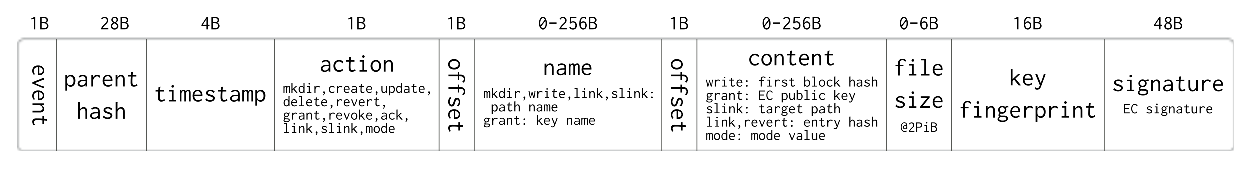
\includegraphics[width=\textwidth]{payload.eps}
\caption{A sample black and white graphic (.eps format)
that has been resized with the \texttt{epsfig} command.}
\label{entrypacket}
\end{figure*}


\begin{enumerate}
\item The hash function of choice is SHA-224, the smallest SHA (28B) considered secure\footnote{\href{https://en.wikipedia.org/wiki/SHA-2\#Comparison\_of\_SHA\_functions}}.
\item We use elliptic curve cryptography with 192bits key size (equivalent to a 2048b RSA key\footnote{\href{https://tools.ietf.org/html/draft-ietf-msec-mikey-ecc-03}}). Keys of this size produce  48 Bytes signatures.
\item File size value is limited to 6 bytes, restricting the maximum file size to 2 PiB.
\item Even though text protocols are easier to work with, we choose to use a more space-efficient binary representation of the entry fields. When possible, field delimitation is based on the field size. Otherwise, a dedicated offset byte is used, which can delimit up to 256byte, just enough to comply with our 256 character upper limit on names.
\end{enumerate}

% TODO diff algorithm comparaisson
Even though the efforts made compacting log entries, log blocks are another story. Updates uses bsdiff4 \link algorithm, which produces a very space-efficient binary diff of two files. Therefore, most of the updates will fit into a single Serf event. However, if updates are big they will not. Fortunately, configuration files are small. In order to have a better understanding of how many events are needed in worst-case scenarios we have characterize the /etc directory of a few Linux system, since all the results are very similar we only present the results of a web server running Debian in figure \ref{characterization}

full state sync disemination probability 1

\begin{figure}
\centering
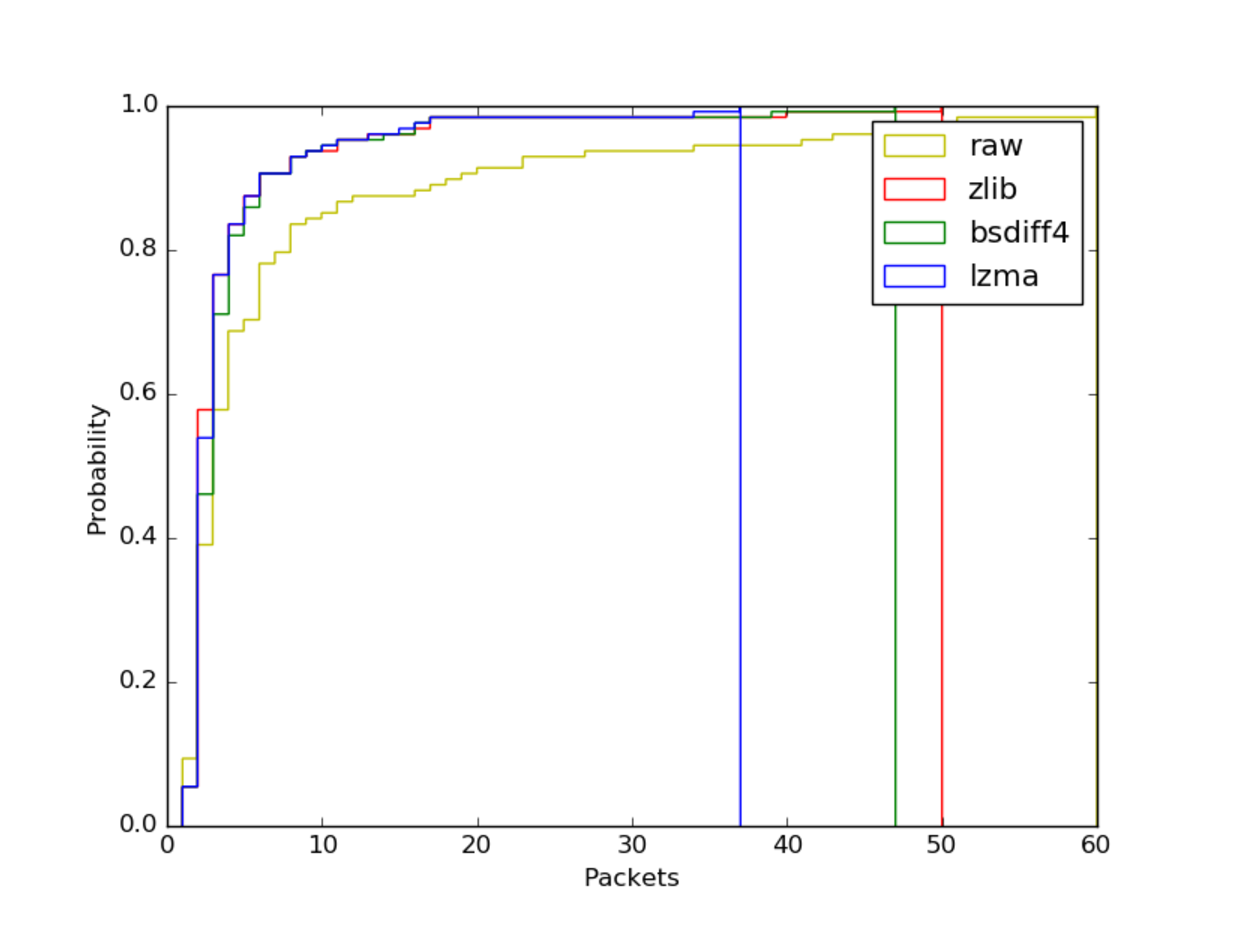
\includegraphics[width=\columnwidth]{characterization.eps}
\caption{A sample black and white graphic (.eps format)
that has been resized with the \texttt{epsfig} command.}
\end{figure}



% todo characterization


They are used for maintaining cluster membership and for broadcasting short events to all the cluster members.

BaseFS uses Serf, a tool for cluster membership, failure detection, and orchestration that is decentralized, fault-tolerant and highly available.


cluster membership and event broadcast a gossip protocol

[1]http://citeseerx.ist.psu.edu/viewdoc/summary?doi=10.1.1.160.2604

a) cluster membership maintenance, b) failure detection and recovery of members and c) broadcast of short events to a cluster.



Gossip protocols, in general and serf in particular, have been useful for two tasks: membership maintenance and broadcast of short events (usually of the size of a UDP packet). The properties that enable:

\item scale well in number of nodes, the number of messages stays constant as nodes are added. 
\item strong completeness of crashed-failing nodes
\item speed of failure detection
\item accuracy


re very efficient and accurate on maintaining cluster membership and detecting failling nodes.


\subsubsection{Synchronization Protocol}

While gossip produces the initial spread of information, a full state synchronization protocol is run infrequently in order to deal with nodes rejoining the cluster after being partitioned, or when a failed node is replaced or partially recovered. Additionally, because the number of blocks sent through the gossip layer is limited, a mechanism to spread remaining blocks is needed.

In order to make the information exchange during replica synchronization efficient, BaseFS uses Merkle trees. Data is hashed at multiple levels of granularity and nodes can quickly find out which part of the data is divergent. The Merkle tree is built conforming to the filesystem hierarchy. Each path hash is computed recursively, using the XOR of its sub-paths as well as its own related entries. The root path is the XOR of all the log entries. The protocol communication is an iterative process, walking and expanding those paths with a mismatching hash. Nodes will detect divergence and interchange log entries and blocks until they are fully synchronized.

The block hashes are not included on the Merkle tree. Doing so will make the synchronization protocol very unstable during periods of gossip dissemination. The root hash will flap its value very rapidly. To avoid this effect, as well as preventing nodes to simultaneously retrieve the same blocks from multiple peers, we introduce the notion of \textit{block state}. Files can be in one of the following three states:

\begin{itemize}
\item Receiving - indicates an initial state, the node has received a new \textit{write} entry. The sync protocol will announce this file as being received, no change performed to the Merkle tree.
\item Stalled - a file enters this state when no related block has been received after some time $t$. Both, the entry hash and the last received block are added to the Merkle tree.
\item Completed - all related blocks have been received. The \textit{Entry} hash is included to the Merkle tree. In case the previous state was stalled, the last block hash is removed.
\end{itemize}


% TODO state machine of the sync state

\begin{figure}
\centering
\begin{BVerbatim}
Receiving:  No hash
Completed:  Entry hash
Stalled:    Entry hash and last block hash
       +-----------+       ehash
[i]--->| Receiving +------------+
       +---+-------+            |
           |   ^          +-----v-----+
     bhash |   | bhash    | Completed |
     ehash |   | ehash    +-----------+
           v   |                ^
        +------+--+       bhash |
        | Stalled +-------------+
        +---------+
\end{BVerbatim}
\caption{C++ code}
\end{figure}

The synchronization protocol is a text-based streaming protocol, using new line characters as delimiters and encoding binary information (block content) in base64. Its alphabet is:

\begin{itemize}
\item \texttt{HASH} - Filesystem root hash. Only sync when equal TODO REPHRASE
\item \texttt{LS} - Path list, includes all path entry hashes, sub-paths hashes and the last-block hash of incomplete files.
\item \texttt{PATH\_REQ} - Path request, indicates a node is missing an entire path and requests all its content to its peer.
\item \texttt{ENTRY\_REQ} - Entry request, used by a node to request a missing entry to its peer.
\item \texttt{BLOCK\_REQ} - idem for blocks
\item \texttt{ENTRIES} - Contains a log entry, can be a response to an \texttt{ENTRY\_REQ} or when a node finds out that its peer is missing some entry.
\item \texttt{BLOCKS} - idem for blocks
\item \texttt{BLOCKS\_REC} - A node announces files in receiving state. In case of divergence the peer can apply this hash to the Merkle tree.
\item \texttt{CLOSE} - Indicates a node is fully synchronize with its peer and communication is terminated.
\item \texttt{EOF} - End of transmission. TODO
\end{itemize}


The pattern of communication is probabilistic, nodes have some probability $p$ of attempting to synchronize with each other. Every $t$ seconds, each node picks a node to communicate with. To initiate synchronization nodes send a \texttt{HASH} and \texttt{LS /} requests containing their own state, and things continue from there.



\section{Implementation}

\item \textbf{Filesystem} - The emulation of filesystem operations on \textit{view} operations. Described in \ref{filesystem}.



Diagram of the modules

BaseFS makes extensive use of concurrency including processes, threads and an event loop. The FUSE interface runs on the main Python thread, as required by its implementation. The Serf agent runs on a separated Python process, and we talk with it using Serf own RPC protocol. We spawn an additional thread for the event loop. Implemented with asyncio, the event loop handles all the remaining network communication in a non-blocking fashion, including the sync protocol, receiving of custom gossip events and commands sent by BaseFS CLI utility. The event loop thread shares memory with the main FUSE thread, and only a single instance of the View has to be maintained, saving memory and computation time.

File Handler also spawns a new process for each registered handler script

\subsection{Filesystem}
The filesystem layer is implemented using FUSE Python bindings\footnote{\href{https://github.com/terencehonles/fusepy}}. FUSE stands for Filesystem in Userspace, and Wikipedia defines it as "an operating system mechanism for Unix-like computer operating systems that lets non-privileged users create their own filesystems without editing kernel code". This is achieved by running filesystem code in user space while the FUSE module provides only a "bridge" to the actual kernel interfaces. The implementation is very straightforward, and almost limited to \textit{View} operations.


The filesystem, however, needs to be aware of new changes made by other nodes. Because of its cost, the \textit{view layer} does not rebuild automatically when new changes arrive. Instead each time we want to read something, the filesystem layer checks if its log seek value is up-to-date with the actual log seek value. A mismatch indicates new entries have arrive and a rebuild of the \textit{view} is performed before doing the actual read.

Another detail worth mentioning is the caching layer used for file write operations. Because the blabla we cluster writes so we can do diff, and safe staff

\subsubsection{Watchers}
The naive approach for applications to react to changes is periodic reading (pulling) the state they are interested in. Modern Linux kernels provide support for filesystem notifications via the inotify subsystem. Unfortunately FUSE is missing support for triggering those events. Since the main objective of BaseFS is to act as a middleware providing shared state between applications, contribute and effective mechanisms that allow applications to react to state changes is very convenient. Support for executing scripts in response to new log entries is natively provided in the form of event handlers.

Event handlers are registered on mounting time and can be any executable, including piped executables (such as \texttt{awk '{print \$2}' | grep foo}), since event handlers are invoked within the context of a shell. The event handler is executed anytime a new log entry is stored. Context for the scripts is given by \texttt{BASEFS\_EVENT\_TYPE} and \texttt{BASEFS\_EVENT\_PATH} environment variables. 


\subsection{Commands}

\begin{verbatim}
Usage: basefs COMMAND [arg...]
       basefs [ --help | -v | --version ]

Basically Available, Soft state, Eventually consistent File System.

Commands:
    mount	Mount an existing filesystem
    run		Run an existing filesystem without mounting it (testing)
    bootstrap	Create a new self-contained filesystem
    genkey	Generate a new EC private key
    keys	List keys and their directories
    grant	Grant key write permission
    revoke	Revoke key write permission
    list	List all available logs
    show	Show a log file using a tree representation
    revert	Revert object to previous state, 'log' command lists all revisions
    blocks	Block state
    members	List cluster members
    serf	Serf RPC Command proxy
    get		Get log from peer address
    installserf	Download and install Serf
    resources	Display BaseFS resource consumption in real-time
    help

Run 'basefs COMMAND --help' for more information on a command
\end{verbatim}


\section{Evaluation}

For the test setup, a set of UNIX shell and Expect scripts 
was designed to automate the testing and ensure each run was 
handled consistently. The Expect scripts began by configuring 
the network emulator, via its XML-RPC interface, to the 
desired delay, line rate constraints, and bit error per packet 
rate. The Expect script would then spawn a tcpdump packet 
capture of all the test traffic by listening on the network 
emulator interface’s connected to the receiver. It would then 
remotely connect to the source and destination nodes via SSH 
and execute the protocol executables for the desired protocol 
implementation run. Once the run was complete, it would tear 
down the spawned processes and loop back around for another 
run if necessary
disemination
correlation




best sync mechansim: random or seed after write

balanced load on the nodes (is the traffic per node even?)
talk about our methodology and approach, reference to other benchmarks (serf?) get inspired by other papers evaluating DS. 

conflicts probability? Low I hope

maybe merge with basefs design (support the design decissions with evidence))

IPFS vs BaseFS ?

gossip layer saturation limit
etc characterization
    bsdiff (designed for executables) ram hungry: bsdiff is quite memory-hungry. It requires max(17*n,9*n+m)+O(1) bytes of memory, where n is the size of the old file and m is the size of the new file. bspatch requires n+m+O(1) bytes.

A note about our implementation, we use highly concurrent design featuring processes, threads and event loops. performance of async core, talk a little bit here
convergence time of sync protocol
convergence time gosssip layer
Fs memory and time vs ext4 or other filesystems: iotests (networked vs single node tests)
NAT resistance

confine tests
locality aware sync protocol based on serf coordinates
and locality in terms of network hops?



\section{The Future}


Some nice features have been left out of the scope of this project, just because our focus has been to proof that our idea works and has meaningful value.

Multiple diff algorithms for diffing, maybe let user choose.
diff of large files, don't put them in memory: fs mount option?

enabler for decentralizate cloud platforms

for simplicity we used next hash -> but introduce merklize infohashes is best

gossip layer problems: Keep track of bad behaviour and ban bad nodes.

sync protocol room for imporvement: biased instead of rand uniformly distributed
For small files it is not really important to give incentives for sharing because the resources that each node has to contribute for becoming part of the network are small. However for large files or very-very large file systemes we can consider to incentive mechanisms:
    a) block-market swarn: write content contains all the blocks hashes of that file, the original content has to be fetched from a bitTorrent-like swarm, much like swaptorrent works (ipfs)
    b) nodes do not contribute all the missing parts when syncing, they can keep track of the behaviour of the other nodes and decide to choke them if appropiate

more than cluster management

a. decentralized state
    Dropbox-like applications: each user with each folder, and shared folders
    SO upgrade on large clusters
    shared configuration for decentralized cloud computing: zookeeper, etcd
    shared in-memory-state for clusters: memcached

b. mutable P2P content
    Mutable P2P file sharing, ok for small files, but incentive mechanissm to avoid free-riders and block sharing swarm may be needed (WRITE magnetlink).
    Live documents: enciclopedia or discographies that self-update when new updates are available

c. monotonicity
    Version control system

Notice that file contents nor metadata (size, name, date) are not encrypted in anyway. Privacy is left intentionally out of the scope of this project since our focus is to prove that our idea works. 


Biased getPeer(randomize algorithm) : network proximity, published new content
imporve serf membership maintenance: when a failing node is remove from the member list?
If baUery power, bandwidth, and other resources are scarce, selfish users may not wish to forward packets for other users
\section{Conclusions}

we presented a system with properties that enables more than decentralize configuration.%\end{document}  % This is where a 'short' article might terminate

%
% The following two commands are all you need in the
% initial runs of your .tex file to
% produce the bibliography for the citations in your paper.
\bibliographystyle{abbrv}
\bibliography{sigproc}  % sigproc.bib is the name of the Bibliography in this case
% You must have a proper ".bib" file
%  and remember to run:
% latex bibtex latex latex
% to resolve all references
%
% ACM needs 'a single self-contained file'!
%
%APPENDICES are optional
%\balancecolumns
%\balancecolumns % GM June 2007
% That's all folks!
\end{document}

